\documentclass[tikz]{standalone}

\usepackage{tikz}
\usepackage{ifthen}
\pgfdeclarelayer{back}
\pgfsetlayers{back,main}

%
% Customize colors
%
\definecolor{chapter-color}{cmyk}{1, 0.50, 0, 0.25}
\definecolor{link-color}{cmyk}{1, 0.50, 0, 0.25}
\definecolor{cite-color}{cmyk}{0, 0.7, 0.9, 0.2}
\definecolor{codegreen}{rgb}{0,0.6,0}
\definecolor{codegray}{rgb}{0.5,0.5,0.5}
\definecolor{codepurple}{rgb}{0.58,0,0.82}
\definecolor{backcolour}{rgb}{0.95,0.95,0.92}
\definecolor{codebgcolor}{RGB}{129, 139, 152}
\definecolor{codehighlightcolor}{RGB}{255, 230, 153}
%\definecolor{codegreen}{RGB}{0, 153, 0}
%\definecolor{codegray}{RGB}{127, 127, 127}
\definecolor{codeblue}{RGB}{102, 214, 237}
\definecolor{codekeyword}{RGB}{249, 36, 114}
\definecolor{codecomment}{RGB}{127, 127, 127}
\definecolor{backcolor}{RGB}{242, 242, 235}
\definecolor{linkcolor}{RGB}{102, 0, 0}
\definecolor{corange}{RGB}{255, 70, 0}
\definecolor{cyellow}{RGB}{209, 153, 0}
\definecolor{cblue}{RGB}{64, 128, 255}
\definecolor{cbrown}{RGB}{153, 102, 51}
\definecolor{cpink}{RGB}{255, 0, 255}
\definecolor{cred}{RGB}{255, 64, 0}
\definecolor{cgreen}{RGB}{0, 191, 0}
\definecolor{clightblue}{RGB}{191, 217, 255}
\definecolor{cturquois}{RGB}{0, 255, 255}
\definecolor{cpurple}{RGB}{128, 0, 255}
\definecolor{clightgreen}{RGB}{175, 255, 175}
\definecolor{clightgray}{RGB}{211, 211, 211}
\definecolor{clightpink}{RGB}{255, 175, 255}
\definecolor{cdarkblue}{RGB}{0, 0, 255}
\definecolor{cdarkred}{RGB}{255, 0, 0}
\definecolor{cdarkgreen}{RGB}{0, 255, 0}
\definecolor{cgray}{RGB}{153, 153, 153}

\definecolor{myblue}{RGB}{55, 126, 184}
\definecolor{myorange}{RGB}{255, 127, 0}
\definecolor{myred}{RGB}{228, 26, 28}
\definecolor{mypurple}{RGB}{152, 78, 163}
\definecolor{mygreen}{RGB}{77, 175, 74}
\definecolor{myyellow}{RGB}{255, 255, 51}
\definecolor{mybrown}{RGB}{166, 86, 40}
\definecolor{mypink}{RGB}{166, 86, 40}
\definecolor{mygray}{RGB}{153, 153, 153}


\colorlet{colorL0}{myorange}
\colorlet{colorL1}{mygreen}
\colorlet{colorL2}{myred}
\colorlet{colorL3}{mypurple}

\makeatletter
\pgfkeys{%
  /tikz/on layer/.code={
    \def\tikz@path@do@at@end{\endpgfonlayer\endgroup\tikz@path@do@at@end}%
    \pgfonlayer{#1}\begingroup%
  }%
}
\makeatother

\begin{document}

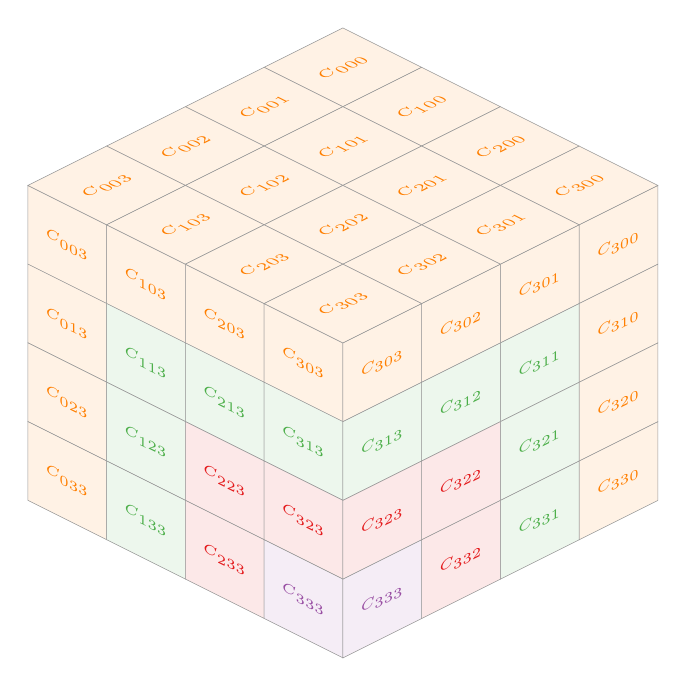
\begin{tikzpicture}

\tikzstyle{every node}=[font=\tiny, text=gray]
%\draw[black, thick] (-0.1,-0.1) rectangle (4.1,4.1);

\def\z{3}%
\begin{scope}[every node/.append style={yslant=-0.5},yslant=-0.5]
\foreach \x in {0,...,3} {
    \foreach \y in {0,...,3} {
        \coordinate (A1) at (\x*1.0+0.0,7.0-\y*1.0);
        \coordinate (B1) at (\x*1.0+1.0,8.0-\y*1.0);

        \ifthenelse{\x=0 \OR \y=0}{
            \draw[color=mygray, fill=colorL0!10, very thin] (A1) rectangle (B1)
                node[midway, color=colorL0]{$C_{\x\y\z}$};
        }{
            \ifthenelse{\x=1 \OR \y=1}{
                \draw[color=mygray, fill=colorL1!10, very thin] (A1) rectangle (B1)
                    node[midway, color=colorL1]{$C_{\x\y\z}$};
            }{
                \ifthenelse{\x=2 \OR \y=2}{
                    \draw[color=mygray, fill=colorL2!10, very thin] (A1) rectangle (B1)
                        node[midway, color=colorL2]{$C_{\x\y\z}$};
                }{
                    \ifthenelse{\x=3 \OR \y=3}{
                        \draw[color=mygray, fill=colorL3!10, very thin] (A1) rectangle (B1)
                            node[midway, color=colorL3]{$C_{\x\y\z}$};
                    }{
                        \ifthenelse{\x=5 \AND \y=5}{
                            \draw[color=white] (A1) rectangle (B1)
                                node[midway, color=mygray]{$\ddots$};
                        }{
                            \ifthenelse{\x=6 \AND \y=6}{
                                \draw[color=white] (A1) rectangle (B1)
                                    node[midway, color=mygray]{$\ddots$};
                            };
                        };
                    };
                };
            };
        };
    };
};
\end{scope}

\def\x{3}%
\begin{scope}[every node/.append style={yslant=0.5},yslant=0.5,shift={(4*1.0,-4*1.0)}]
\foreach \y in {0,...,3} {
    \foreach \z in {0,...,3} {
        \coordinate (A1) at (3*1.0-\z*1.0+0.0, 7.0-\y*1.0);
        \coordinate (B1) at (3*1.0-\z*1.0+1.0, 8.0-\y*1.0);

        \ifthenelse{\y=0 \OR \z=0}{
            \draw[color=mygray, fill=colorL0!10, very thin] (A1) rectangle (B1)
                node[midway, color=colorL0]{$C_{\x\y\z}$};
        }{
            \ifthenelse{\y=1 \OR \z=1}{
                \draw[color=mygray, fill=colorL1!10, very thin] (A1) rectangle (B1)
                    node[midway, color=colorL1]{$C_{\x\y\z}$};
            }{
                \ifthenelse{\y=2 \OR \z=2}{
                    \draw[color=mygray, fill=colorL2!10, very thin] (A1) rectangle (B1)
                        node[midway, color=colorL2]{$C_{\x\y\z}$};
                }{
                    \ifthenelse{\y=3 \OR \z=3}{
                        \draw[color=mygray, fill=colorL3!10, very thin] (A1) rectangle (B1)
                            node[midway, color=colorL3]{$C_{\x\y\z}$};
                    }{
                        \ifthenelse{\y=5 \AND \z=5}{
                            \draw[color=white] (A1) rectangle (B1)
                                node[midway, color=mygray]{$\ddots$};
                        }{
                            \ifthenelse{\y=6 \AND \z=6}{
                                \draw[color=white] (A1) rectangle (B1)
                                    node[midway, color=mygray]{$\ddots$};
                            };
                        };
                    };
                };
            };
        };
    };
};
\end{scope}

\def\y{0}%
\begin{scope}[every node/.append style={yslant=0.5,xslant=-1},yslant=0.5,xslant=-1,shift={(8*1.0,0*1.0)}]
\foreach \x in {0,...,3} {
  \foreach \z in {0,...,3} {
    \coordinate (A1) at (3*1.0-\z*1.0+0.0,7.0-\x*1.0);
    \coordinate (B1) at (3*1.0-\z*1.0+1.0,8.0-\x*1.0);

    \draw[color=mygray, fill=colorL0!10, very thin] (A1) rectangle (B1)
        node[midway, color=colorL0]{$C_{\x\y\z}$};
  };
};
\end{scope}


\end{tikzpicture}

\end{document}